%%%%%%%%%%%%%%%%%%%%%%%%%%%%%%%%%%%%%%%%%%%%%%%%%%%%%%%%%%%%%%%%%%%%%%%%%%%%
% AGUJournalTemplate.tex: this template file is for articles formatted with LaTeX
%
% This file includes commands and instructions
% given in the order necessary to produce a final output that will
% satisfy AGU requirements, including customized APA reference formatting.
%
% You may copy this file and give it your
% article name, and enter your text.
%
%
% Step 1: Set the \documentclass
%
% There are two options for article format:
%
% PLEASE USE THE DRAFT OPTION TO SUBMIT YOUR PAPERS.
% The draft option produces double spaced output.
%

%% To submit your paper:
\documentclass[draft]{agujournal2019}
\usepackage{url} %this package should fix any errors with URLs in refs.
\usepackage{lineno}
\usepackage{color}
\graphicspath{ {figures/} }
\linenumbers
%%%%%%%
% As of 2018 we recommend use of the TrackChanges package to mark revisions.
% The trackchanges package adds five new LaTeX commands:
%
%  \note[editor]{The note}
%  \annote[editor]{Text to annotate}{The note}
%  \add[editor]{Text to add}
%  \remove[editor]{Text to remove}
%  \change[editor]{Text to remove}{Text to add}
%
% complete documentation is here: http://trackchanges.sourceforge.net/
%%%%%%%

\draftfalse

\journalname{JGR: Space Physics}


\begin{document}

\title{Statistical Properties of Curtain Electron Precipitation Dervied with AeroCube-6}

%% ------------------------------------------------------------------------ %%
%
%  AUTHORS AND AFFILIATIONS
%
%% ------------------------------------------------------------------------ %%

\authors{M. Shumko\affil{1}, A.T. Johnson\affil{1}, J.G. Sample\affil{1}, D.L. Turner\affil{3}, T.P. O'Brien\affil{2}, and J.B. Blake\affil{2}}


\affiliation{1}{Department of Physics, Montana State University, Bozeman, Montana, USA}
\affiliation{2}{Space Science Applications Laboratory, The Aerospace Corportation, El Segundo, California USA}
\affiliation{3}{Johns Hopkins Applied Physics Laboratory, Laurel, Maryland, USA}

\correspondingauthor{M. Shumko}{msshumko@gmail.com}

\begin{keypoints}
\item We used the dual AeroCube-6 CubeSats to identify stationary, narrow, and persistent $>30$ keV precipitation in low Earth orbit
\item A single low Earth-orbiting spacecraft can easily misidentify curtains as microburst precipitation
\item A few curtains actively precipitated for at least six seconds
\end{keypoints}

%% ------------------------------------------------------------------------ %%
%
%  ABSTRACT
%
% A good abstract will begin with a short description of the problem
% being addressed, briefly describe the new data or analyses, then
% briefly states the main conclusion(s) and how they are supported and
% uncertainties.
%% ------------------------------------------------------------------------ %%

%% \begin{abstract} starts the second page

\begin{abstract}
yeah
\end{abstract}

\section{Plain Language Summary}
\textcolor{blue}{
Outline
\begin{enumerate}
\item Stuff
\end{enumerate}
}

\section{Introduction}

\section{Instrumentation} \label{instrumentation}

\section{Methodology} 
\subsection{Curtain Identification} \label{curtain_identification}

\begin{figure}
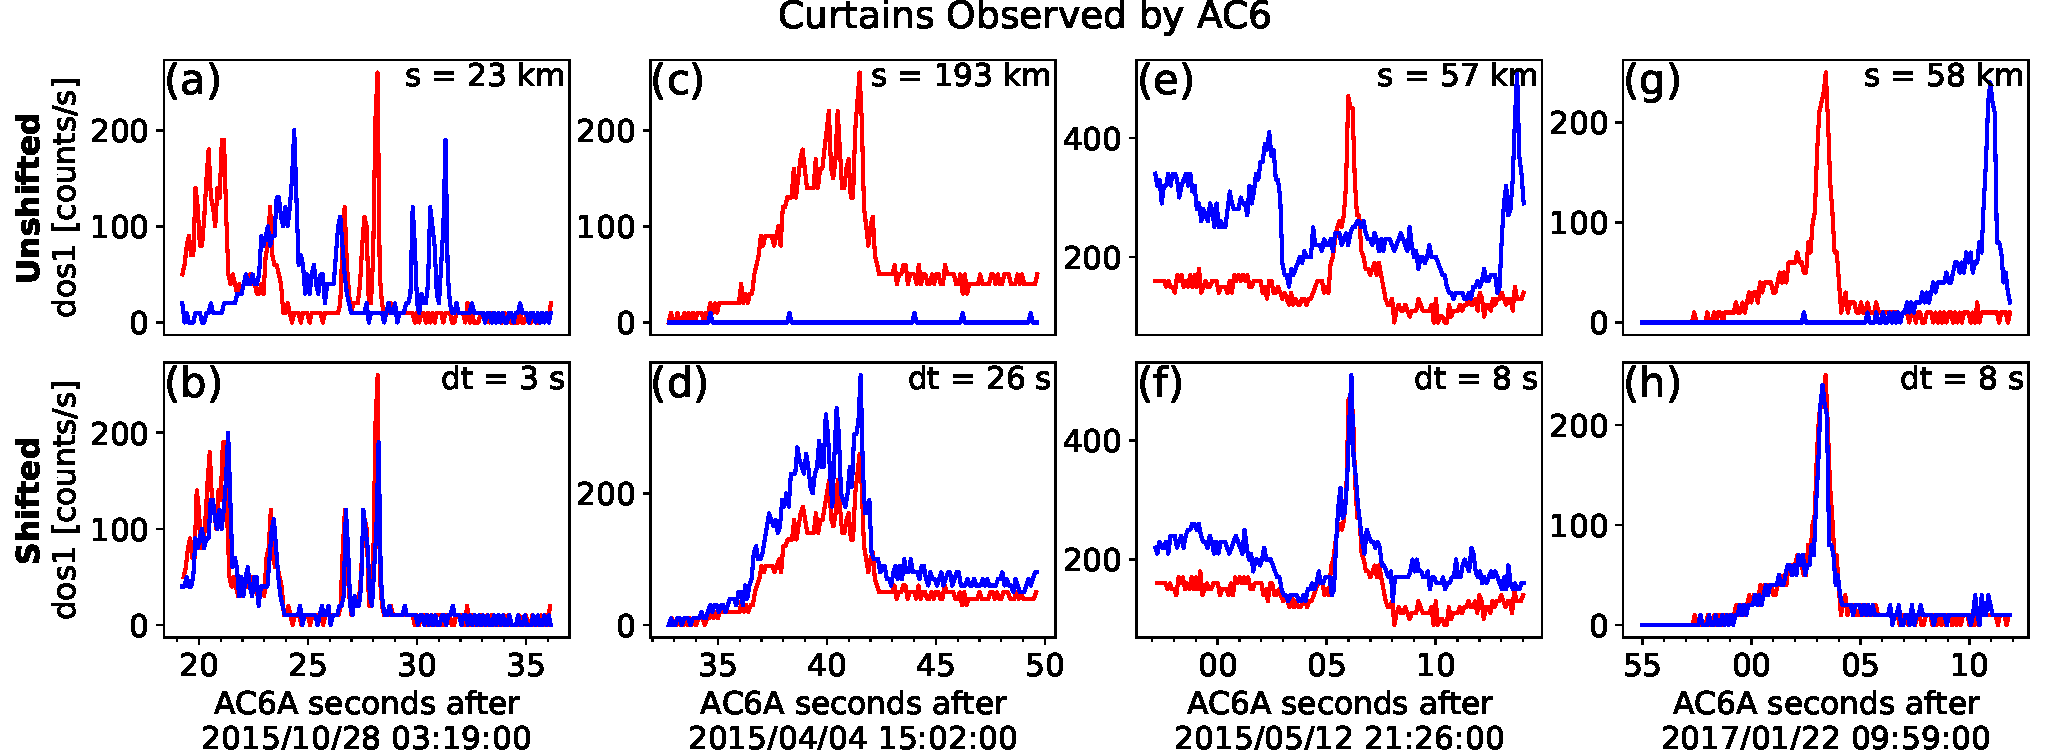
\includegraphics[width=\textwidth]{fig1.pdf}
\caption{Four examples showing the AC6 $> 30$ keV electron data taken by AC6 at the same time in the top row and at the same position in the bottom row. To show the data at the same position the time series data from one spacecraft was shifted by the in-track lag and annotated by dt. These examples show curtain precipitation highly correlated for up to 26 seconds.}
\label{fig1}
\end{figure}

\section{Results}
\subsection{Curtain Statistics} \label{stats}

\subsection{Local Curtain Precipitation}

\section{Discussion} \label{discussion}
text

\section{Conclusions}
text

% \appendix

\acknowledgments
This work was made possible with the help from the many engineers and scientists at The Aerospace Corporation who designed, built, and operated AC6. M. Shumko was supported by NASA Headquarters under the NASA Earth and Space Science Fellowship Program - Grant 80NSSC18K1204. D.L. Turner is thankful for support from the Van Allen Probes mission and a NASA grant (Prime award number: 80NSSC19K0280). The work at The Aerospace Corporation was supported in part by RBSP-ECT funding provided by JHU/APL contract 967399 under NASA's Prime contract NAS501072. The AC6 data is available at http://rbspgway.jhuapl.edu/ac6 and the IRBEM-Lib version used for this analysis can be downloaded from https://sourceforge.net/p/irbem/code/616/tree/.

Title: Statistical Properties of Curtains--Latitudinally-Narrow and Persistent Electron Precipitation Phenomena

This study leverages AC6, a multi-spacecraft mission, to interpret and understand particle precipitation in a way that is impossible with a single spacecraft.

This study leverages the asymmetry in Earth's magnetic field. The asymmetric magnetic field results in the SAA and the BLC, two very related and unique regions

Particles that impact the atmosphere are lost during that bounce motion. We found curtains in the bounce loss cone, a region in the North Atlantic near and above Iceland.

The bounce loss cone is magnetically connected to the SAA, where Earth's magnetic field is weakest near Earth's surface. A particle observed in the blc in the northern hemisphere will descend below 100 km altitude. At sub-100 km altitudes the particle has a high chance of encountering and scattering with the atmosphere and be lost. 

We found curtain elections that, when given the chance to execute their cyclical bounce motion, will descend below Earth's surface in the SAA. An election can not survive that trip.

Write the paper and ask the question: "What is this paper really about?" Not just curtains, but uncovering something unexpected that has been observed and overlooked for decades.

Are curtains related to aurora? This is a good question---one that is not pertinent here (idea from The Elements of Style p.68).

Sections:
- Introduction
- instrumentation
- curtain identification
- statistical properties
- what are curtains?
- discussion and conclusion

\bibliography{/home/mike/Dropbox/0_firebird_research/A_presentations/refs}
\bibliography{"refs"}

\end{document}